% $Id: template.tex 11 2007-04-03 22:25:53Z jpeltier $

\documentclass{vgtc}                          % final (conference style)
%\documentclass[review]{vgtc}                 % review
%\documentclass[widereview]{vgtc}             % wide-spaced review
%\documentclass[preprint]{vgtc}               % preprint
%\documentclass[electronic]{vgtc}             % electronic version

%% Uncomment one of the lines above depending on where your paper is
%% in the conference process. ``review'' and ``widereview'' are for review
%% submission, ``preprint'' is for pre-publication, and the final version
%% doesn't use a specific qualifier. Further, ``electronic'' includes
%% hyperreferences for more convenient online viewing.

%% Please use one of the ``review'' options in combination with the
%% assigned online id (see below) ONLY if your paper uses a double blind
%% review process. Some conferences, like IEEE Vis and InfoVis, have NOT
%% in the past.

%% Figures should be in CMYK or Grey scale format, otherwise, colour 
%% shifting may occur during the printing process.

%% These few lines make a distinction between latex and pdflatex calls and they
%% bring in essential packages for graphics and font handling.
%% Note that due to the \DeclareGraphicsExtensions{} call it is no longer necessary
%% to provide the the path and extension of a graphics file:
%% \includegraphics{diamondrule} is completely sufficient.
%%
\ifpdf%                                % if we use pdflatex
  \pdfoutput=1\relax                   % create PDFs from pdfLaTeX
  \pdfcompresslevel=9                  % PDF Compression
  \pdfoptionpdfminorversion=7          % create PDF 1.7
  \ExecuteOptions{pdftex}
  \usepackage{graphicx}                % allow us to embed graphics files
  \DeclareGraphicsExtensions{.pdf,.png,.jpg,.jpeg} % for pdflatex we expect .pdf, .png, or .jpg files
\else%                                 % else we use pure latex
  \ExecuteOptions{dvips}
  \usepackage{graphicx}                % allow us to embed graphics files
  \DeclareGraphicsExtensions{.eps}     % for pure latex we expect eps files
\fi%

%% it is recomended to use ``\autoref{sec:bla}'' instead of ``Fig.~\ref{sec:bla}''
\graphicspath{{figures/}{pictures/}{images/}{./}} % where to search for the images

\usepackage{microtype}                 % use micro-typography (slightly more compact, better to read)
\PassOptionsToPackage{warn}{textcomp}  % to address font issues with \textrightarrow
\usepackage{textcomp}                  % use better special symbols
\usepackage{mathptmx}                  % use matching math font
\usepackage{times}                     % we use Times as the main font
\renewcommand*\ttdefault{txtt}         % a nicer typewriter font
\usepackage{cite}                      % needed to automatically sort the references
\usepackage{tabu}                      % only used for the table example
\usepackage{booktabs}                  % only used for the table example

\usepackage{float}
%% We encourage the use of mathptmx for consistent usage of times font
%% throughout the proceedings. However, if you encounter conflicts
%% with other math-related packages, you may want to disable it.


%% If you are submitting a paper to a conference for review with a double
%% blind reviewing process, please replace the value ``0'' below with your
%% OnlineID. Otherwise, you may safely leave it at ``0''.
\onlineid{0}

%% declare the category of your paper, only shown in review mode
\vgtccategory{Research}

%% allow for this line if you want the electronic option to work properly
\vgtcinsertpkg

%% In preprint mode you may define your own headline.
%\preprinttext{To appear in an IEEE VGTC sponsored conference.}

%% Paper title.

\title{The Causal Link Detective Game}

%% This is how authors are specified in the conference style

%% Author and Affiliation (single author).
%%\author{Roy G. Biv\thanks{e-mail: roy.g.biv@aol.com}}
%%\affiliation{\scriptsize Allied Widgets Research}

%% Author and Affiliation (multiple authors with single affiliations).
%%\author{Roy G. Biv\thanks{e-mail: roy.g.biv@aol.com} %
%%\and Ed Grimley\thanks{e-mail:ed.grimley@aol.com} %
%%\and Martha Stewart\thanks{e-mail:martha.stewart@marthastewart.com}}
%%\affiliation{\scriptsize Martha Stewart Enterprises \\ Microsoft Research}

%% Author and Affiliation (multiple authors with multiple affiliations)
\author{Abhijat Shrivastava \\ %
        \scriptsize abhijat.shrivastava@stonybrook.edu %
\and Trisha Kanji\\ %
     \scriptsize trisha.kanji@stonybrook.edu }

%% Abstract section.
\abstract{

The Causal Link Detective Game is an interactive tool that provides users the authority to incorporate additions/changes to an existing causal graph visualization presented, such that the final result makes more sense in terms of the real-world data. 
It presents the user with an initial causal model and allows them to verify the model's credibility using personal intellect and further suggest the possibility of new latent variables that would complete the causal model with valid causal relations.

} 
% end of abstract
\CCScatlist{
  \CCScatTwelve{Causal Analysis}{Visu\-al\-iza\-tion}{Visu\-al\-iza\-tion techniques}{SEM Analysis};
  \CCScatTwelve{Structural Equation Modelling}{Visu\-al\-iza\-tion}{Causal Link Detection and evaluation methods}{}
}
%%%%%%%%%%%%%%%%%%%%%%%%%%%%%%%%%%%%%%%%%%%%%%%%%%%%%%%%%%%%%%%%
%%%%%%%%%%%%%%%%%%%%%% START OF THE PAPER %%%%%%%%%%%%%%%%%%%%%%
%%%%%%%%%%%%%%%%%%%%%%%%%%%%%%%%%%%%%%%%%%%%%%%%%%%%%%%%%%%%%%%%%

\begin{document}

\firstsection{Introduction}

\maketitle

Deriving exact causal relations between two variables is a difficult task due to the possible incompleteness of the data and the context. It is difficult to identify if among two correlated variables there exists a causal relation, which variable is the cause and which one is the effect. Also, another possibility could be the existence of an external variable not present in the data set, which has the same cause-effect relationship for both the given variables being examined. Without any contextual information, it is not possible to determine the cause-effect relationship between two variables.
\\[1em]

For example, the ongoing COVID19 disease has multiple symptoms like cough, fever etc. But it cannot be inferred directly that a person is suffering from COVID19 just because they are suffering from cough and cold. There is something missing in this relation. If the person has recently travelled to/from the countries affected, and the person is sick, then it can be inferred that he/she might be suffering from Coronavirus. Clearly, the addition of a new variable “Recent travel” in the data is capable of changing the way people might interpret the data.
\\[1em]

We aim to extract such relations and provide the users with a game-like interface, using which they can put their domain knowledge and extract relevant data from the web which can be fed to the tool, to identify the actual causal relations. If the data is incomplete, the facts derived may not be representative of the actual causal relation between certain data fields. For example, a data set consisting of only 2 fields: ‘SAT score’ and ‘Income’ might result in a causal model which suggests that high income leads to high SAT score. This is not entirely true, since there might be various other additional factors that actually contribute to getting a high SAT score. The application will allow the user to look out for these variables, which might be missing from the current data set but might be available in some other data sets, which can be added to build a credible causal model. %

\section{Work Done}
Given a data set, we ask the user to select the variables they want to be included in the causal model. 

\begin{figure}[H]
  \caption{Variable selection screen}
  \centering
  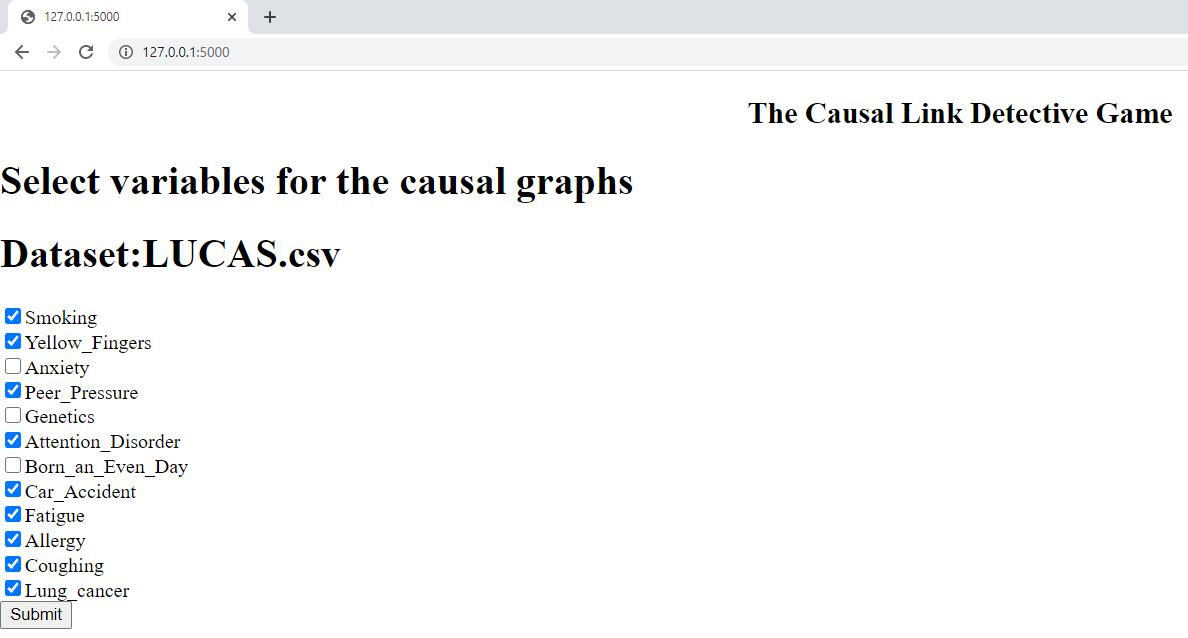
\includegraphics[width=0.5\textwidth]{s1}
\end{figure}


From these variables, we generate a potential causal model 'M' of the data set using the Tetrad tool and pyCausal module in Python for generating causal models. The algorithm used by Tetrad for our scenario is 'FGES' (Fast Greedy Equivalence Search). From this model 'M', we generate 4 different sub graphs and display them to the user interface. 
\\[1em]
We also provide the user with the correlation matrix displayed in the form of a heatmap. This heatmap shows how all pairs of variables are correlated with each other. A shade of red indicates negative correlation, and a shade of green indicates a positive correlation. The strength of the shade represents the strength of the correlation.
\\[1em]
The user, based on their expertise of the domain of the data set as well as looking at the provided heatmap, can select the best looking causal model out of the four and start working on it.

\begin{figure}[H]
  \caption{Sub-graph selection screen}
  \centering
  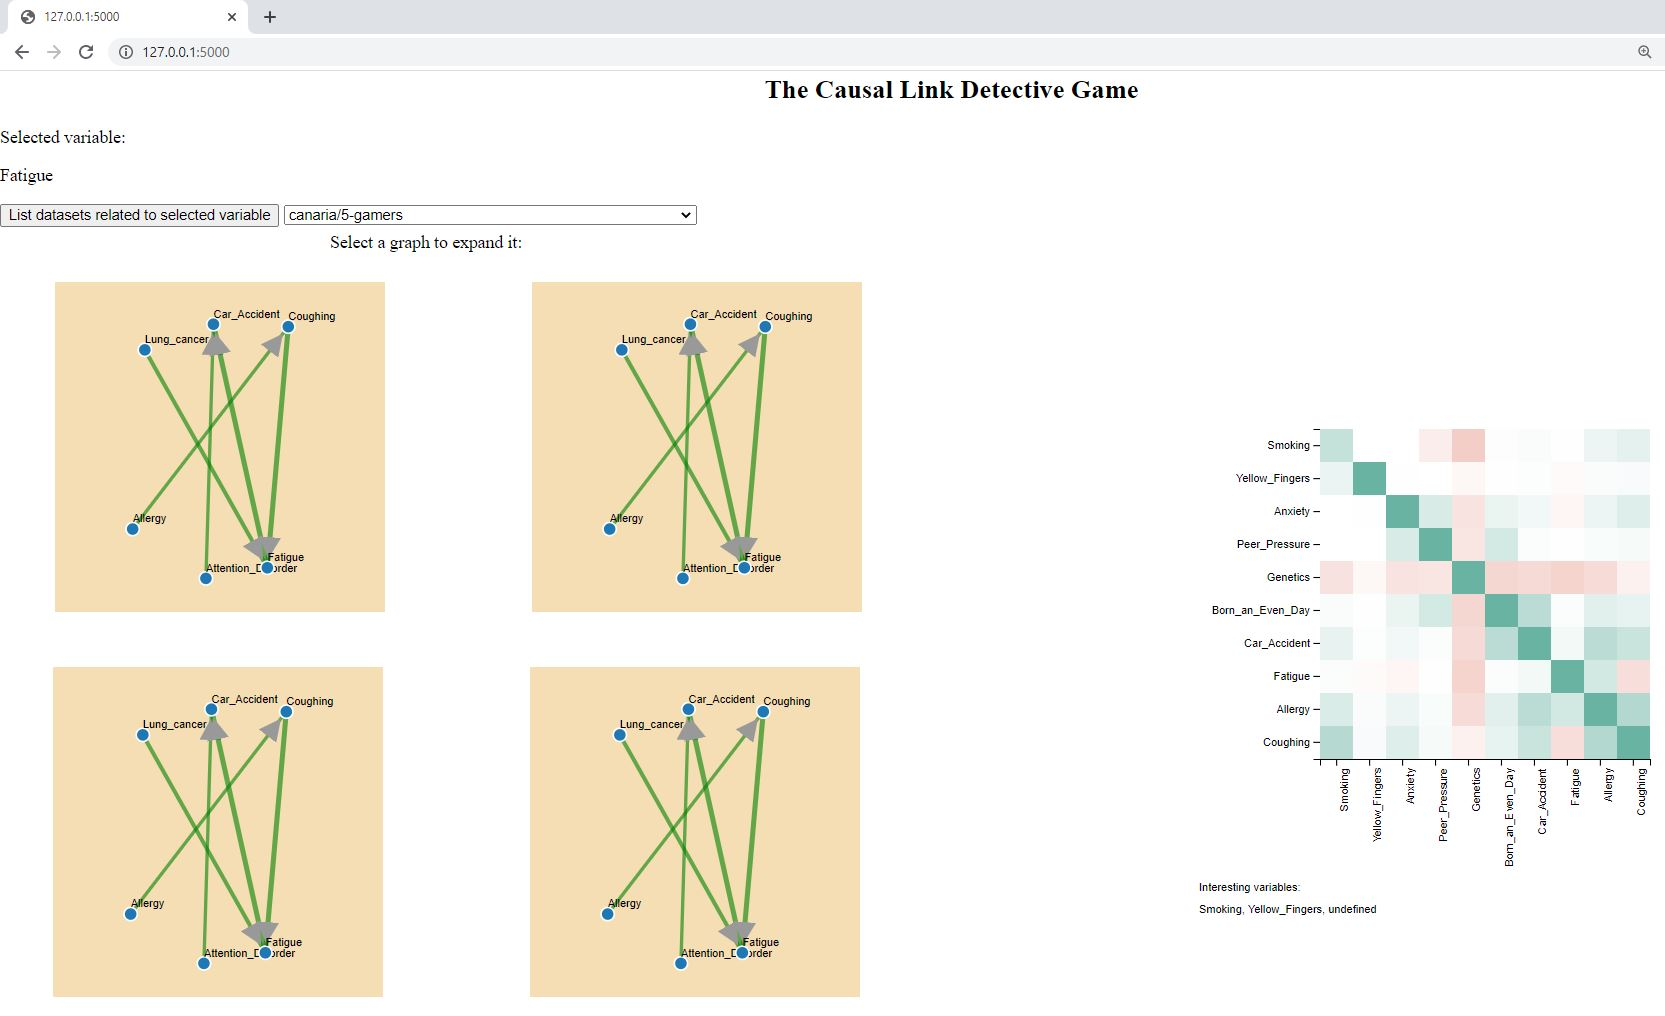
\includegraphics[width=0.5\textwidth]{s2}
\end{figure}


The user is provided with a dynamic causal graph to which the user can make the following changes:
Add an edge between two nodes, reverse an edge between two nodes, remove a node, remove an edge, add an unused variable from the data set.
After each of these actions, the user is provided with dynamic feedback about the fit of the model using the following metrics: BIC, Chi-squared test, CFI and RMSEA.
After making a change to the causal graph, if a particular metric value is better than before, it is displayed in green. If it is worse than before, then it is displayed in red. If it is same as before (no change), then it is displayed in black.
\\[1em]

We also give the user feedback about some models similar to the one the user is working with. This gives the user an idea about which direction they should be going for.

\begin{figure}[H]
  \caption{Playing with the causal model and getting dynamic feedback}
  \centering
  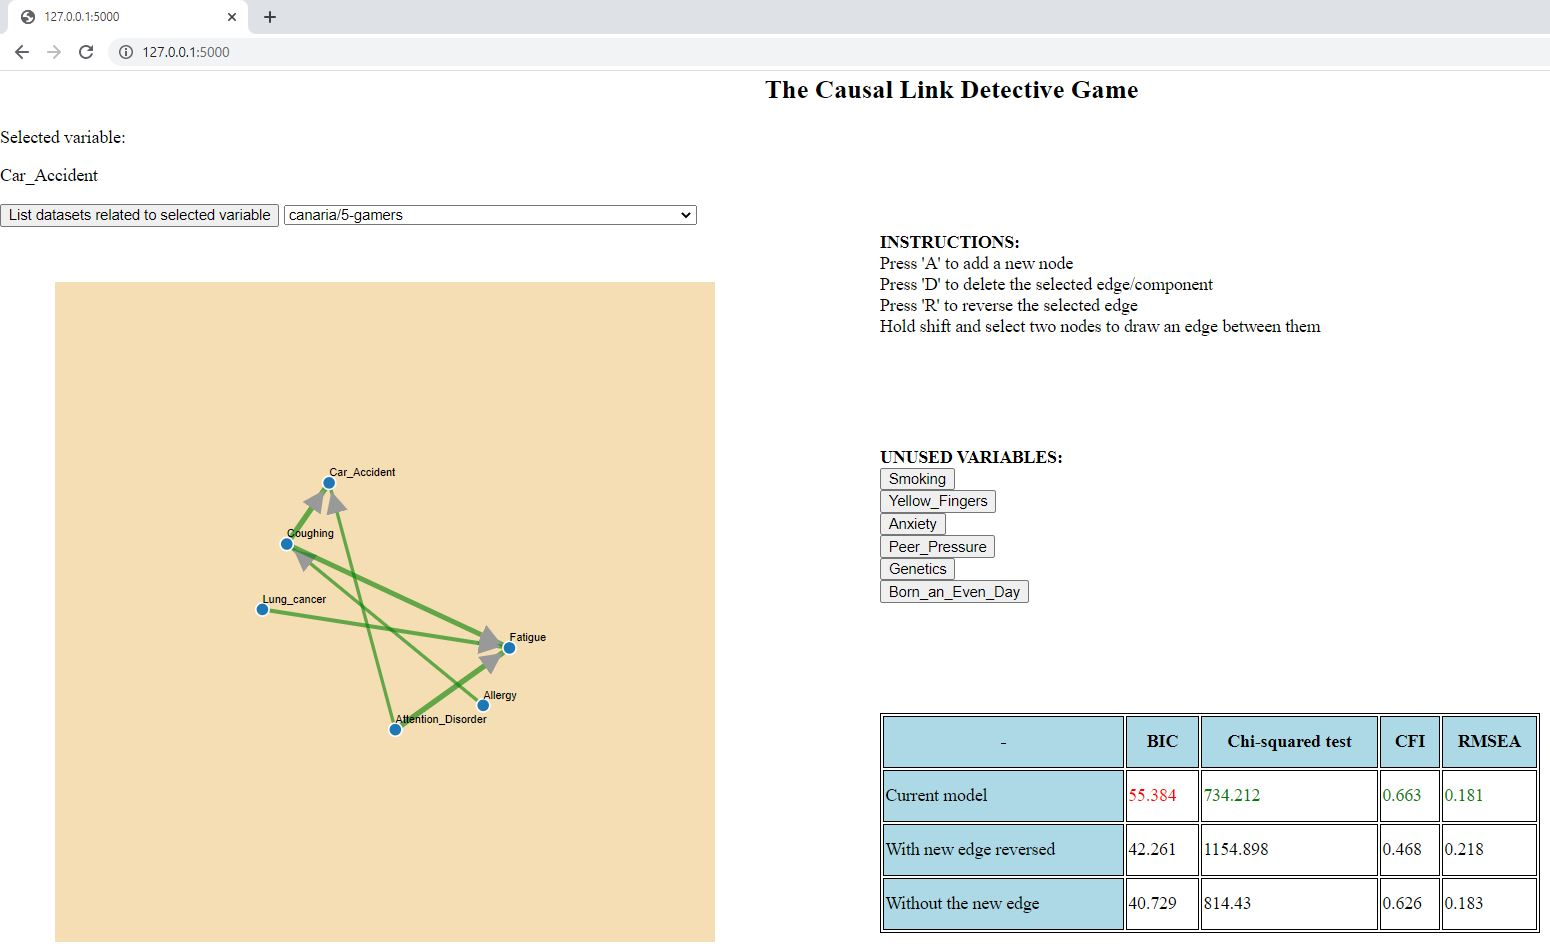
\includegraphics[width=0.5\textwidth]{s3}
\end{figure}

We have also incorporated a "search string" feature, which shows the user the list of available Kaggle datasets which are in a way related to the current dataset's selected variable. When the user selects one of these datasets from the list, the new dataset gets downloaded to the user's system and the user can inspect it to get a better understanding of the causal network.
\\[1em]
We have used D3.js and Python to make this tool. We have used Flask to connect the frontend to the backend service and used Semopy to evaluate the causal models. Figure1, Figure2 and Figure3 depict the different windows of our user interface.



\section{Model Analysis using Structural Equation Modeling (SEM)}

Generally, traditional statistical methods utilize just one statistical test to determine the significance of the analysis. Structural Equation Modeling, however, relies on several statistical tests to determine the adequacy of model fit to the data. This makes it more reliable to be used.

Formal statistical tests and fit indices have been developed in order to see how well the proposed model fits the driving theory. Because different measures of fit capture different elements of the fit of the model, it would be appropriate to report a selection of different fit measures.  A model is considered to be a good fit if the value of the Chi-squared test is insignificant, and at least one incremental fit index (like CFI, GFI, TLI, AGFI, etc.) and one badness of fit index (like RMR, RMSEA, SRMR, etc.) meets the predetermined criteria.
In our case study, we have used some of the most commonly used measures of fit to assess our causal graphs, described as follows.

\begin {itemize}
\item Bayesian Information Criterion (BIC)
\paragraph{}
The Bayesian Information Criterion (BIC) is a statistical measure to quantify the model performance by scoring it based on its log-likelihood and complexity.
The BIC score for model selection is minimized, i.e. the model with the lowest BIC should be selected. 


$BIC = ln(n) k - 2 ln(\hat{L})$  where,
\newline
$\hat{L}$ : maximized value of the likelihood function of the model
\newline
n: number of parameters
\newline
k: number of free parameters to be estimated
\paragraph{}
However, a limitation of BIC, that we need to keep in account is that they cannot handle complex collections of models and do not take the uncertainty of the models into account and thus sometimes end-up selecting models that are too simple.

 

\item Chi-squared test
\paragraph{}
The chi-squared test indicates the amount of difference between expected and observed co-variance matrices. It is a fundamental measure of fit used in the calculation of many other fit measures. A chi-squared value close to zero indicates little difference between the expected and observed co-variance matrices. In addition, the probability level must be greater than 0.05 when chi-square is close to zero. Chi-square is a “badness-of-fit” index, meaning smaller values indicate better fit.

\item Comparative Fit Index (CFI)
\paragraph{}
The Comparative Fit Index (CFI) is equal to the discrepancy function adjusted for sample size.
In examining baseline comparisons, the CFI depends in large part on the average size of the correlations in the data. If the average correlation between variables is not high, then the CFI will not be very high. A CFI value of 0.95 or higher is desirable.
CFI ranges from 0 to 1, with a larger value indicating better model fit. Acceptable model fit is indicated by a CFI value of 0.95 or greater. CFI is a “goodness-of-fit” index where larger values mean better fit.
 
 
\item Root Mean Square Error of Approximation (RMSEA)
\paragraph{}
Root Mean Square Error of Approximation (RMSEA) is related to residual in the model and is used for accommodating large sample sizes.
RMSEA values range from 0 to 1 with a smaller RMSEA value indicating better model fit.
RMSEA is a fit index where a value of zero indicates the best fit. While the guideline for determining a "close fit" using RMSEA is highly contested, most researchers concur that an RMSEA of 0.1 or more indicates poor fit. Acceptable model fit is indicated by an RMSEA value of 0.06 or less. 
\end{itemize}

\section{CASE STUDY}

For our case study, we considered the case of Lung Cancer and its causes. We used our Causal Link Detective Game tool on the LUCAS (Lung Cancer Simple set) dataset to analyze the relationship between it's variables. It contains artificially generated data which is generated by causal Bayesian networks with binary variables. It consists of the boolean variables like Smoking, Yellow Fingers, Anxiety, Attention Disorder,Born on Even Day,Car Accident, Fatigue, Allergy, Coughing, Lung Cancer etc.

\subsection{Implementation / Interface Details}

The interface allows the user to pick a subset of these variables, out of which they want their causal model to be constructed. It further presents the user with four smaller sub graphs of this causal model in separate windows to choose from and analyze. These sub graphs will have at  most 5 random variables from the initial set marked by the user and will present the initial causal model of the selected data set that our causal inference engine deems to be fit. The causal inference engine basically refers to the causal algorithm responsible for building the causal model.
\\[0.5em]
Our interface utilizes the TETRAD tool and the Py Causal python module under the TETRAD Project repository by the Center for Causal Discovery (CCD), which offers tools for wrapping algorithms for performing causal discovery on big data and contains
a variety of well-tested algorithms for searching for causal explanations of data under a variety of data formats and user knowledge of the domain.
\\[1em]
Once the user selects the sub graph which they want to analyze, the selected graph is displayed in a new window along with a list of so far unused variables for the user to experiment with. The sub graph is presented as an interactive force directed layout which allows the user to add/remove/reverse edges and/or add/delete nodes(variables). This allows the user to experiment with various use cases of different causal relations which the user finds to be fitting. This means that the user can also introduce latent variables to the model (with one of the three possibilities out of Chains, Collider and Fork relation), in order to improve the causal model such that this latent variable brings out the hidden causalities in the model.
\\[1em]
As the user keeps on modifying the graph, the interface keeps on running the causal inference engine for each instance and depicts the model parameters in a table adjacent to the interactive graph. We use SEM evaluation as the statistical analysis technique to analyze our causal relationships and model. We use the semopy package in Python which stands for Structural Equation Models Optimization in Python and is designed to help employ SEM techniques for analyzing models. 
\\[1em]
Using this, we predict the BIC, Chi-Squared Test, CFI and RMSEA values for each of the models, so that the user can verify statistically the significance of the new model generated. Additionally, upon adding a new edge, the table also lists the values for the model with the edge reversed and the initial model state without the edge, so that the user can analyze the impact of adding new relationships and whether the new model generated is stable or not.


\subsection{Results/ Analysis}

There are three ways in which a user could improve the existing causal model presented to them, namely by adding latent variables to the graph, by reversing existing causal relations and/or by removing redundant variables or causal relations present in the graph.

Here, by latent variable, we refer to a hypothetical construct that is invoked to explain observed co-variation in behavior. Further, the new latent variable has the possibility of forming one of the following three relationships, with the already existing (potentially causal) relation:
\begin{itemize}
    \item Chain: Infers that the new latent variable forms a chain like relation where the initial source variable causes the latent variable and the initial target variable is caused by the latent variable. (see Figure4)
    \item Fork: Infers that the latent variable introduced causes both the initial source and target variables. (see Figure4)
    \begin{figure}[tb]
     \centering % avoid the use of \begin{center}...\end{center} and use \centering instead (more compact)
     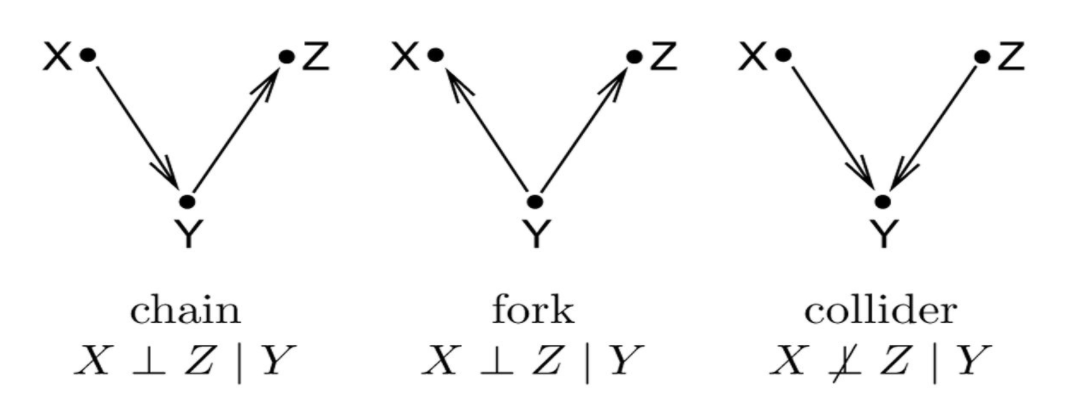
\includegraphics[width=\columnwidth]{CFC}
     \caption{Visualization of three types of Latent Variable relations}
     
     \label{fig:sample}
    \end{figure}
    \item Collider: Infers that new latent variable is in fact caused by both the source and the target variables in the initial causal graph. (see Figure4)
\end{itemize}




The following sections describe the different use cases using example causal graphs and include detailed analysis of the models obtained. The user is initially presented with the LUCAS data set variables and is presented with a set of variables to choose from for the initial sub graphs. 

\subsubsection{Add Latent Variable to existing causal graph}
\begin{itemize}
    \item Chain Relation: Figure5 shows the initial causal graph, indicating that Peer Pressure causes anxiety. In Figure6 we add smoking as the new latent variable to the causal graph, as intrinsically peer pressure might result in a person smoking, in which case smoking would be attributing to their anxiety. In order to verify our instinct, we refer to the corresponding model performance scores in Table 1 (page 5). Here we see that the new model's BIC drops significantly to 0.8604 from 20.4684 on introducing chain relationship with smoking as the latent variable. Also, CFI increases from 1.0992 to 7.8065 and even if the RMSEA of the new model is increasing, the value of 0.0584 is within the accepted value of 0.06.

    \begin{figure}[H]
      \caption{Case: Add (chain) before adding edge}
      \centering
      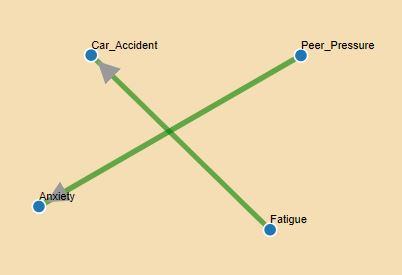
\includegraphics[width=0.4\textwidth]{c1_1}
    \end{figure}
    
    \begin{figure}[H]
      \caption{Case: Add (chain) after adding edge}
      \centering
      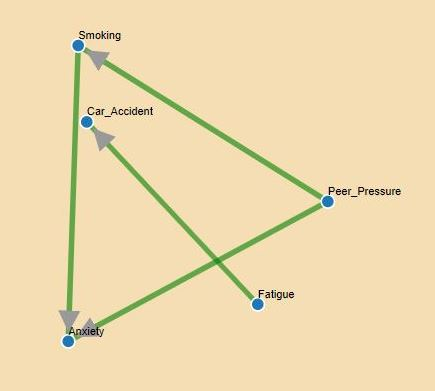
\includegraphics[width=0.4\textwidth]{c1_2}
    \end{figure}

    \item Fork Relation: Figure7 shows the initial causal graph presented by the interface upon selecting variables. This model indicates that Fatigue causes Attention Disorder. We figure that there might be an underlying factor that might be causing both fatigue and attention disorder, which is anxiety. 
    \\[1em]
    We introduce the latent variable anxiety to the model and add edges from anxiety to both Fatigue and Attention Disorder as shown in Figure8. Upon comparing the model fit parameters, we choose the new model over the previous one. Even though the BIC for the second model is quite higher, we suggest this might be because of the increased complexity of the model as BIC penalizes the model for that. Also, the second model is chosen as its RMSEA value falls in the accepted value range of 0.00-0.06, while the first model's RMSEA is well over 0.06. Even if the CFI value has dropped for this model, it is well above the threshold value of 0.95 and thus can be accepted. 

    
    
    \begin{figure}[H]
      \caption{Case: Add (fork) before adding edge}
      \centering
      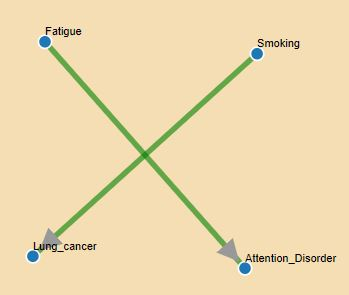
\includegraphics[width=0.4\textwidth]{c2_1}
    \end{figure}
    
    \begin{figure}[H]
      \caption{Case: Add (fork) after adding edge}
      \centering
      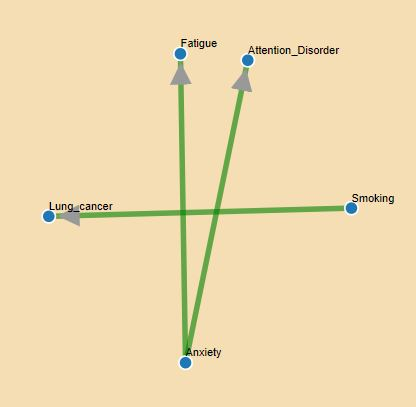
\includegraphics[width=0.4\textwidth]{c2_2}
    \end{figure}
    
    \item Collider Relation: As we can see in Figure9, the initial causal graph obtained using the shown four variables depict that Smoking causes Genetics, which intuitively does not make any sense. Instead, we think of a latent variable which might have hidden relations with both genetics and smoking. Including the variable Lung Cancer in the existing model makes more sense from our perspective, as Genetics and Smoking might be the primary reasons causing Lung Cancer. Following our instincts, we add an edge pointing to Lung Cancer from both Genetics and Smoking and assess the model parameters. Referring to Table1 (page 5), we see that the BIC and Chi-squared values decrease and the RMSEA value is well within the accepted value of 0.06. Even if the CFI value has dropped for this model, it is well above the threshold value of 0.95 and thus can be accepted. 
    
    \begin{figure}[H]
      \caption{Case: Add (collider) before adding edge}
      \centering
      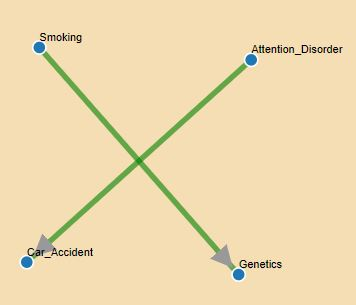
\includegraphics[width=0.4\textwidth]{c3_1}
    \end{figure}

    \begin{figure}[H]
      \caption{Case: Add (collider) after adding edge}
      \centering
      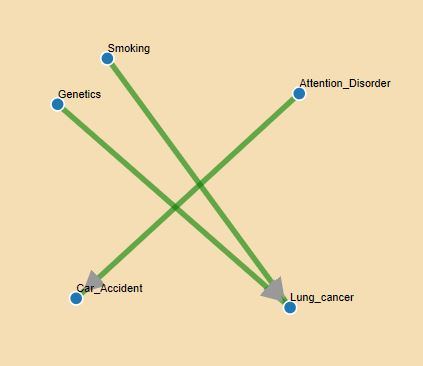
\includegraphics[width=0.4\textwidth]{c3_2}
    \end{figure}
    \end{itemize}



\subsubsection{Modify (Reverse) Existing Causal Relationship}
\paragraph{}
As we can see in the Figure11, the causal model obtained for five variables depicts that Lung Cancer causes Smoking, which fails to make sense in the real world scenario. We figure out that the causal relation should work the other way round, i.e., smoking might result in Lung Cancer. Thus, we asses the model parameters in Table1 (page 5) after reversing this edge. We see a drop in the BIC and Chi-squared values and a significantly lower RMSEA nearing 0. Even if the CFI value has dropped for this model, it is well above the threshold value of 0.95 and thus can be accepted. Thus, we choose the second model with reversed edge.
\begin{figure}[H]
  \caption{Case: Before reversing edge}
  \centering
  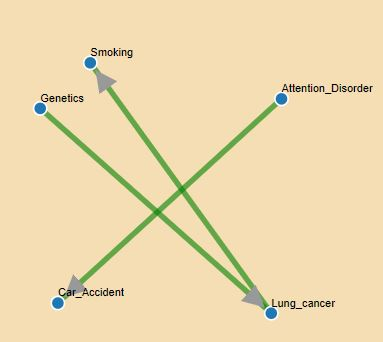
\includegraphics[width=0.4\textwidth]{c4_1}
\end{figure}

\begin{figure}[H]
  \caption{Case: After reversing edge}
  \centering
  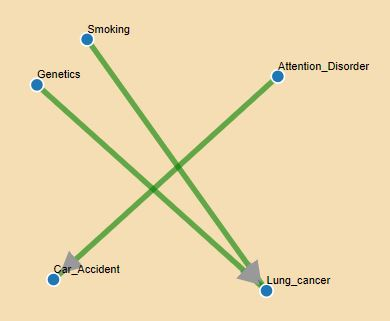
\includegraphics[width=0.4\textwidth]{c4_2}
\end{figure}

\begin{table}[tb]
  \caption{Model performance metrics for causal graph \newline (before and after changes in form of latent variable introduction, reversal of causal relations and removal of redundant relations/variables)}
  \label{tab:vis_papers}
  \scriptsize%
	\centering%
  \begin{tabu}{%
	r%
	*{7}{c}%
	*{2}{r}%
	}
  \toprule
   CASE & \rotatebox{90}{Model Type}  &   \rotatebox{90}{BIC} &   \rotatebox{90}{Chi-squared Test} &   \rotatebox{90}{CFI} &   \rotatebox{90}{RMSEA}   \\
  \midrule
	Add (Chain) & Initial & 20.4684 & 5.4962 & 1.0992 & 0.0070 \\
  Add (Chain) & Modified & 0.8604 & 54.6454 & 7.8065 & 0.0584 \\
  \midrule
  Add (Fork) & Initial & 18.8846 & 239.5670 & 47.9134 & 0.1532 \\
  Add (Fork) & Modified & 53.1103 & 49.3200 & 8.2201  & 0.0600 \\
  \midrule
  Add (Collider) & Initial & 17.5123 & 155.3964 & 31.0793 & 0.1227 \\
  Add (Collider) & Modified & 13.5149 & 15.6369 & 1.7374 & 0.01921 \\
  \midrule
  Reverse Relation & Initial & 24.4464 & 80.6706 & 10.0838 & 0.0674 \\
  Reverse Relation & Modified & 13.5149 & 15.6369 & 1.7374 & 0.01921 \\
  \midrule
  Remove Variable  & Initial & 73.8767 & 401.5621 & 40.1562 & 0.1399 \\
  Remove Variable  & Modified & 53.1103 & 49.3200 & 8.2200 & 0.0601 \\
  \midrule
  Remove Relation  & Initial & 20.4961 & 14.2536 & 1.0964 & 0.0069 \\
  Remove Relation  & Modified & 20.6608 & 55.3308 & 4.2562 & 0.0404 \\

  
%   \textbf{sum} & \textbf{1545} & \textbf{9} & \textbf{632} & \textbf{310} & \textbf{50} & \textbf{123} & \textbf{25} & \textbf{2694} & \textbf{2546} \\
  \bottomrule
  \end{tabu}%
\end{table}

\subsubsection{Remove existing causal relations/ variables}

\begin{itemize}
\item Remove redundant variable: 

    As we can see in Figure13, the initial causal graph of 5 variables presented indicates
    that the variable Born on an Even Day causes Anxiety. However, in a real world scenario, this seems unlikely. Thus, we choose to remove this variable as it seems redundant and holds no significant relation to the other variables. As we refer to Table1 (page 5) for assessing the model parameters, we see decreased values of BIC, Chi-squared and RMSEA (less than 0.06). Even if the CFI value has dropped for this model, it is well above the threshold value of 0.95 and thus can be accepted.
    
    \begin{figure}[H]
      \caption{Case: Before removing redundant variable}
      \centering
      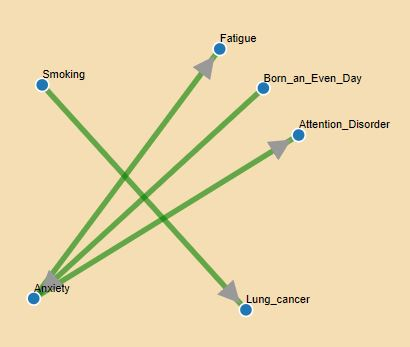
\includegraphics[width=0.4\textwidth]{c5_2}
    \end{figure}
    
    \begin{figure}[H]
      \caption{Case: After removing redundant variable}
      \centering
      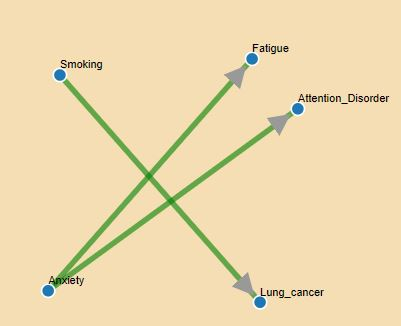
\includegraphics[width=0.4\textwidth]{c5_1}
    \end{figure}
    
    
\item Remove redundant relation
    As we can see in Figure15, the initial causal model of 6 variables depicts an edge from coughing to car accident, which makes little sense. So, we modify this causal graph by deleting this edge and assess the model parameters for the modified graph. Referring  Table1 (page 5), we see a decreased BIC score, low RMSEA within 0.06 and an increased CFI value, leading us to choose the new model.
    
    \begin{figure}[H]
      \caption{Case: Before removing redundant relation}
      \centering
      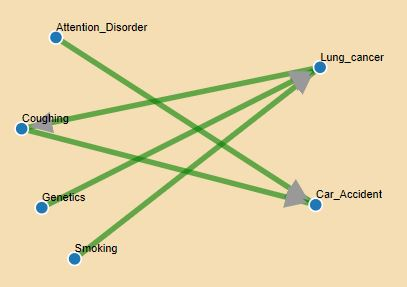
\includegraphics[width=0.4\textwidth]{c6_1}
    \end{figure}
    
    \begin{figure}[H]
      \caption{Case: After removing redundant relation}
      \centering
      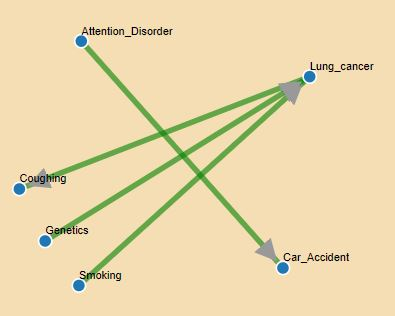
\includegraphics[width=0.4\textwidth]{c6_2}
    \end{figure}
\end{itemize}


\section{Future Work}

\begin{itemize}
\item Currently, the "search string" feature allows us to view all available Kaggle datasets related to the selected variable and automatically download them to our system. However, merging these datasets with the selected dataset is something that needs the datasets to have a common column such as ZIP code. This can be done by limiting the available datasets such that only those datasets are visible which have atleast one common column with the main dataset. In this way, both the datasets can be merged to get a better picture of the causal network.
\item Currently, the entire causal model is evaluated as a whole and the dynamic feedback is displayed to the user. However, a better approach might be to show the user the individual impact of a newly created edge to the causal model. For this, the p-value of the edge can be calculated and displayed along with the edge. This can help the user to more accurately analyze the fit of the model.
\end{itemize}

\section{Conclusion}

Causal analysis is a powerful machine learning tool to derive knowledge about the world from data. Most causal links offer only simplified explanations of the true relationships because of the problem of incomplete data with limited scope. We have aimed to develop an interactive interface to overcome this problem by providing the user an interface to determine the unknown relations and refine the causal model. The interface can be used to perform causal analysis on various important topics of societal interest like education inequality.

%% if specified like this the section will be committed in review mode
\acknowledgments{
We wish to thank Professor Klaus Mueller and Md Naimul Hoque for constantly guiding us in the right direction throughout the project. Their timely advice, meticulous scrutiny along with technical and conceptual guidance have helped us to a great extent to accomplish this task. Their dedication, keen interest and challenging attitude towards us and the project alike has been responsible for the completion of our work.}

% \bibliographystyle{abbrv}
\bibliographystyle{abbrv-doi}
%\bibliographystyle{abbrv-doi-narrow}
%\bibliographystyle{abbrv-doi-hyperref}
%\bibliographystyle{abbrv-doi-hyperref-narrow}


\begin{thebibliography}{9}


\bibitem{Paper} 
Georgy Meshcheryakov, Anna A. Igolkina
\textit{semopy: A Python package for Structural
Equation Modeling}. September 10, 2019
 \\\texttt{https://arxiv.org/pdf/1905.09376.pdf}
  \\\texttt{https://www.tandfonline.com/doi/full/10.1080/10705511.2019.1704289}


\bibitem{Paper} 
Jun Wang, Klaus Mueller
\textit{Visual Causality Analysis Made Practical}. October 2017
 \\\texttt{https://ieeexplore.ieee.org/document/8585647}
 
 \bibitem{Dataset} 
\textit{LUCAS dataset (LUng CAncer Simple set)}
 (http://www.causality.inf.ethz.ch/data/LUCAS.html)
 
  \bibitem{Tetrad} 
\textit{Tetrad Causal tool }
 (https://github.com/bd2kccd/py-causal)
 (https://www.ccd.pitt.edu/tools/)
 
   \bibitem{FGES} 
\textit{Fast Greedy Search (FGES) Algorithm for Discrete Variables }
 (https://www.ccd.pitt.edu//wp-content/uploads/2018/10/FGES1d-user-documentation-7\textunderscore20\textunderscore2016-sample-size.pdf)
 
    \bibitem{FGES} 
\textit{Fast Greedy Search (FGES) Algorithm for Continuous Variables}
 (https://www.ccd.pitt.edu//wp-content/uploads/2018/10/FGES1c-user-documentation-5\textunderscore21\textunderscore2016-sample-size.pdf)
 
 \bibitem{Paper} 
Hu, L. \& Bentler,P.M. 
\textit{Cutoff criteria for fit indexes in co-variance structure analysis: Conventional criteria versus new alternatives. Structural Equation Modeling}. 1999
 \\\texttt{https://psycnet.apa.org/doi/10.1080/10705519909540118}

 
\end{thebibliography}
\end{document}
